\documentclass[11pt,letterpaper]{article}
\usepackage[margin=.9in]{geometry}
\usepackage{graphicx,fontspec,microtype,booktabs,tabularx,array,xcolor,tikz,float,needspace}
\setmainfont{TeX Gyre Pagella}
\usetikzlibrary{arrows.meta,positioning}
\usepackage{xurl,soul}
\usepackage[colorlinks=true,urlcolor=blue!55!black,linkcolor=blue!55!black]{hyperref}
\definecolor{researcher}{HTML}{315B70}
\definecolor{agent}{HTML}{26333D}
\definecolor{model}{HTML}{26333D}
\definecolor{error}{HTML}{26333D}
\definecolor{ink}{HTML}{26333D}
\definecolor{leadhl}{HTML}{E8E8E8}
\definecolor{markhl}{HTML}{E8E8E8}
\definecolor{goodhl}{HTML}{E8E8E8}
\newcommand{\leadmark}[1]{{\sethlcolor{leadhl}\hl{#1}}}
\newcommand{\syntaxmark}[1]{{\sethlcolor{markhl}\hl{#1}}}
\newcommand{\goodmark}[1]{{\sethlcolor{goodhl}\hl{#1}}}
\newcommand{\notenum}[1]{\textsuperscript{\textbf{#1}}}
\newcolumntype{Y}{>{\raggedright\arraybackslash}X}
\setlength{\parskip}{6pt}\setlength{\parindent}{0pt}
\linespread{1.07}
\setlength{\emergencystretch}{2em}
\setlength{\textfloatsep}{16pt}
\title{A Prompted Researcher Simulator for TREC UserSim 2026}
\author{Nidhin Pattaniyil \and Tanwir Zaman \and Semih Yagli}\date{}
\hypersetup{pdftitle={A Prompted Researcher Simulator for TREC UserSim 2026},pdfauthor={Nidhin Pattaniyil, Tanwir Zaman, Semih Yagli}}
% Decorative vector icons; speaker labels remain explicit.
\newcommand{\simicon}{\tikz[baseline=-.55ex,x=1.3ex,y=1.3ex,line width=.6pt]{\draw (.8,1.4) circle (.34);\draw (.1,.1) .. controls (.1,.95) and (1.5,.95) .. (1.5,.1);}}
\newcommand{\searchicon}{\tikz[baseline=-.55ex,x=1.3ex,y=1.3ex,line width=.6pt]{\draw (.65,1) circle (.47);\draw (1,.65)--(1.5,.12);}}

\begin{document}
\begin{center}
{\Large\bfseries A Prompted Researcher Simulator\\[3pt]for TREC UserSim 2026}\par
\vspace{3pt}
{\setlength{\tabcolsep}{9pt}\begin{tabular}{@{}ccc@{}}
Nidhin Pattaniyil & Tanwir Zaman & Semih Yagli\\[2pt]
\footnotesize\href{mailto:npatta01@gmail.com}{npatta01@gmail.com} &
\footnotesize\href{mailto:zaman.tanwir@gmail.com}{zaman.tanwir@gmail.com} &
\footnotesize\href{mailto:semihyagli1@gmail.com}{semihyagli1@gmail.com}
\end{tabular}}\\[4pt]
{\small Independent researchers\enspace$\cdot$\enspace Team NP Labs}
\end{center}
\begin{abstract}
We used GPT-6 Luna~\cite{luna} to play the researcher in both TREC UserSim tasks. One model call drafts a reply; a second edits the wording. In Task 1, the editor can also correct claims that the researcher did something the conversation does not support. In Task 2, it keeps the draft's decision to continue or stop.
\par\smallskip\noindent
Our replies were 80--92\% longer than human replies in the preliminary organizer results. Average human-likeness ratings were 2.38/4 for Task 1 and 2.31/4 for Task 2 on the rated subsets. The editor left 95\% of generated Task 2 drafts unchanged, including some poorly rated replies. We examine the prompt and two recorded conversations to show what the editor left unchanged and what we would change in a future submission.
\end{abstract}

\section{Introduction}
TREC UserSim asks participants to simulate a researcher looking for datasets. The organizers provide the search assistant, and our system produces the researcher's messages~\cite{track}. We participated as NP Labs.

\textbf{Task 1: predict one reply.} Given a researcher profile, goal and partial conversation, produce the next researcher message. The simulator starts from the supplied history for each case.

\textbf{Task 2: run the conversation.} Start from a researcher profile and goal, respond to the organizer's assistant over multiple turns, and decide when to finish or abandon the search (Figure~\ref{fig:tasks}).

\begin{figure}[H]\centering
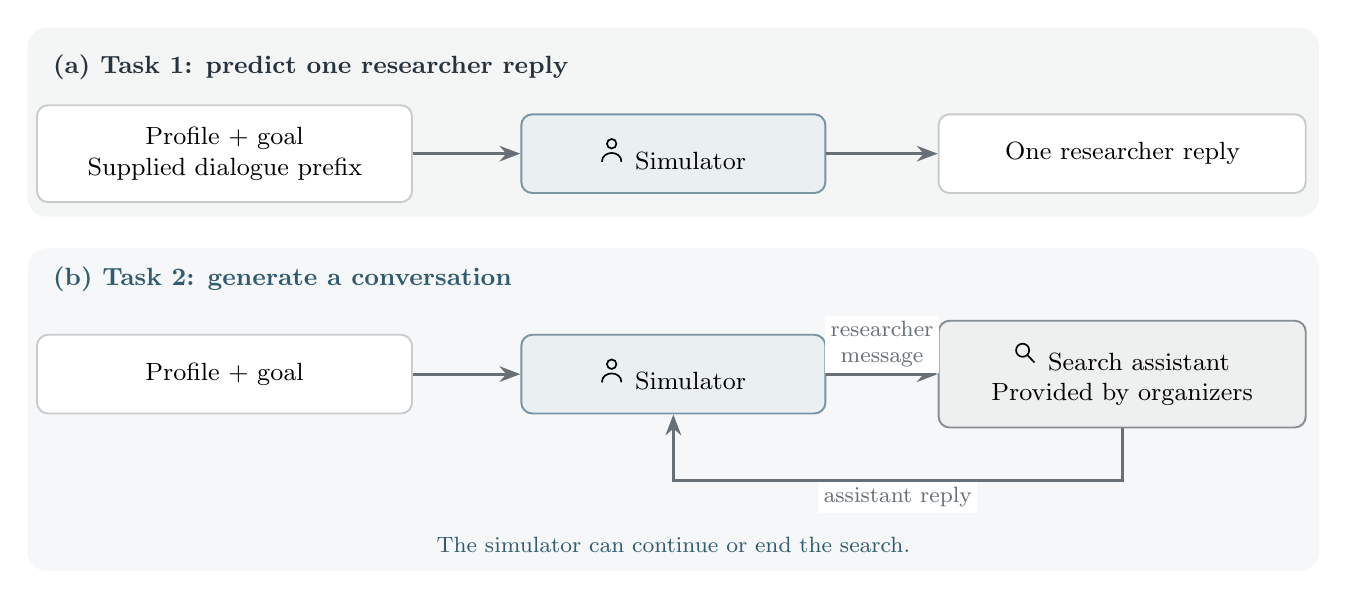
\begin{tikzpicture}[x=1cm,y=1cm,>=Stealth,font=\small,
 box/.style={draw=ink!25,fill=white,rounded corners=4pt,line width=.7pt,inner sep=8pt,align=center,minimum height=1.0cm},
 modelbox/.style={box,draw=researcher!65,fill=researcher!10},
 lab/.style={font=\footnotesize,fill=white,inner sep=2pt,align=center}]
\fill[agent!5,rounded corners=7pt] (-.2,.6) rectangle (16.2,-1.8);
\fill[researcher!5,rounded corners=7pt] (-.2,-2.2) rectangle (16.2,-6.3);
\node[anchor=west,font=\small\bfseries,text=agent] at (0,.1) {(a) Task 1: predict one researcher reply};
\node[box,text width=4.2cm] (context) at (2.3,-1.0) {Profile + goal\\Supplied dialogue prefix};
\node[modelbox,text width=3.3cm] (one) at (8.0,-1.0) {\simicon\enspace Simulator};
\node[box,text width=4.1cm] (reply) at (13.7,-1.0) {One researcher reply};
\draw[->,line width=1pt,color=ink!70] (context.east)--(one.west);
\draw[->,line width=1pt,color=ink!70] (one.east)--(reply.west);

\node[anchor=west,font=\small\bfseries,text=researcher] at (0,-2.6) {(b) Task 2: generate a conversation};
\node[box,text width=4.2cm] (scenario) at (2.3,-3.8) {Profile + goal};
\node[modelbox,text width=3.3cm] (session) at (8.0,-3.8) {\simicon\enspace Simulator};
\node[box,draw=agent!55,fill=agent!8,text width=4.1cm] (agent) at (13.7,-3.8) {\searchicon\enspace Search assistant\\Provided by organizers};
\draw[->,line width=1pt,color=ink!70] (scenario.east)--(session.west);
\draw[->,line width=1pt,color=ink!70] (session.east)--node[lab,above]{researcher\\message} (agent.west);
\draw[->,line width=1pt,color=ink!70] (agent.south)--(13.7,-5.15)--node[lab,below]{assistant reply} (8.0,-5.15)--(session.south);
\node[anchor=north,align=center,font=\footnotesize,text=researcher] at (8.0,-5.75) {The simulator can continue or end the search.};
\end{tikzpicture}

\caption{The simulator writes the researcher's messages. Task 1 asks for one reply; Task 2 continues the exchange with the organizers' assistant.}\label{fig:tasks}
\end{figure}

\section{Method: drafting and editing researcher replies}
For each task, we use GPT-6 Luna to draft a reply and then edit it~\cite{code}. The two calls see the researcher's profile, goal, domain knowledge, known datasets and full conversation history. There is no fine-tuning or retrieval. The draft prompt asks the model to speak naturally as that researcher. In Task 2, it can stop when it has enough help or the search is going nowhere.

The editor uses the last two researcher messages as examples of how to write. In Task 1, it can correct a claim such as ``I downloaded it'' if the researcher's background and earlier messages do not support it. In Task 2, it changes only the wording and keeps the draft's stop decision (Figure~\ref{fig:method}).

\begin{figure}[H]\centering
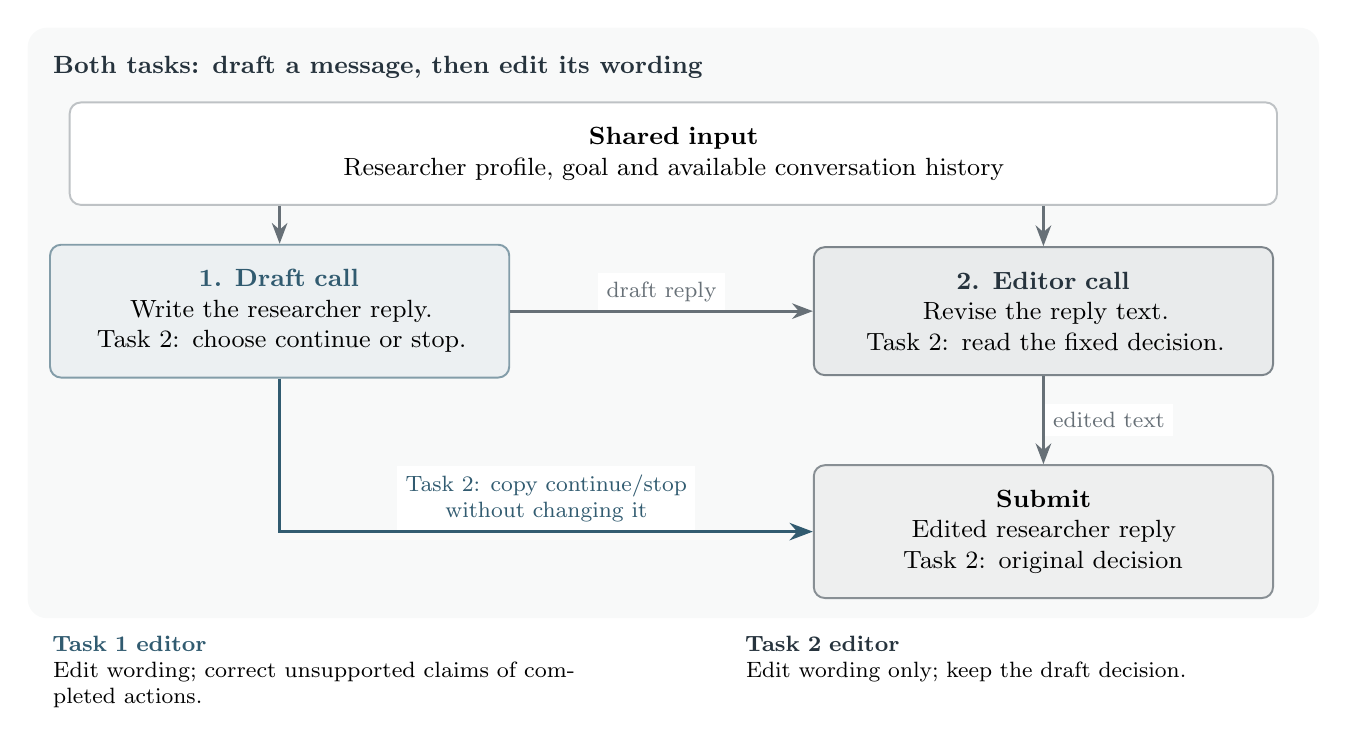
\begin{tikzpicture}[x=1cm,y=1cm,>=Stealth,font=\small,
 box/.style={draw=ink!30,fill=white,rounded corners=4pt,line width=.7pt,inner sep=9pt,align=center},
 call/.style={box,draw=researcher!60,fill=researcher!9,text width=5.2cm,minimum height=1.6cm},
 lab/.style={font=\footnotesize,fill=white,inner sep=3pt,align=center}]
\fill[ink!3,rounded corners=7pt] (-.2,.6) rectangle (16.2,-6.9);
\node[anchor=west,font=\small\bfseries,text=ink] at (0,.1) {Both tasks: draft a message, then edit its wording};
\node[box,draw=ink!30,text width=14.7cm] (context) at (8,-1.0) {\textbf{Shared input}\\Researcher profile, goal and available conversation history};
\node[call] (draft) at (3.0,-3.0) {\textcolor{researcher}{\textbf{1. Draft call}}\\Write the researcher reply.\\Task 2: choose continue or stop.};
\node[call,draw=model!60,fill=model!10] (edit) at (12.7,-3.0) {\textcolor{model}{\textbf{2. Editor call}}\\Revise the reply text.\\Task 2: read the fixed decision.};
\draw[->,line width=1pt,color=ink!70] (draft.north |- context.south)--(draft.north);
\draw[->,line width=1pt,color=ink!70] (edit.north |- context.south)--(edit.north);
\draw[->,line width=1pt,color=ink!70] (draft.east)--node[lab,above]{draft reply} (edit.west);
\node[box,fill=agent!8,draw=agent!55,text width=5.2cm,minimum height=1.1cm] (out) at (12.7,-5.8) {\textbf{Submit}\\Edited researcher reply\\Task 2: original decision};
\draw[->,line width=1pt,color=ink!70] (edit.south)--node[lab,right]{edited text} (out.north);
\draw[->,line width=1.2pt,color=researcher] (draft.south)--(3.0,-5.8)--node[lab,above,text=researcher]{Task 2: copy continue/stop\\without changing it} (out.west);
\node[anchor=north west,text width=7.1cm,align=left,font=\footnotesize] at (0,-7.0) {\textcolor{researcher}{\textbf{Task 1 editor}}\\Edit wording; correct unsupported claims of completed actions.};
\node[anchor=north west,text width=7.1cm,align=left,font=\footnotesize] at (8.8,-7.0) {\textcolor{model}{\textbf{Task 2 editor}}\\Edit wording only; keep the draft decision.};
\end{tikzpicture}

\caption{Our two model calls. In Task 2, the editor sees the draft's stop decision but cannot change it. The final reply carries that original decision.}\label{fig:method}
\end{figure}

We wanted the reply to sound more like the researcher without changing what they asked for. We therefore told the editor to make small changes and keep the details (Figure~\ref{fig:prompt}).

\begin{figure}[H]\centering
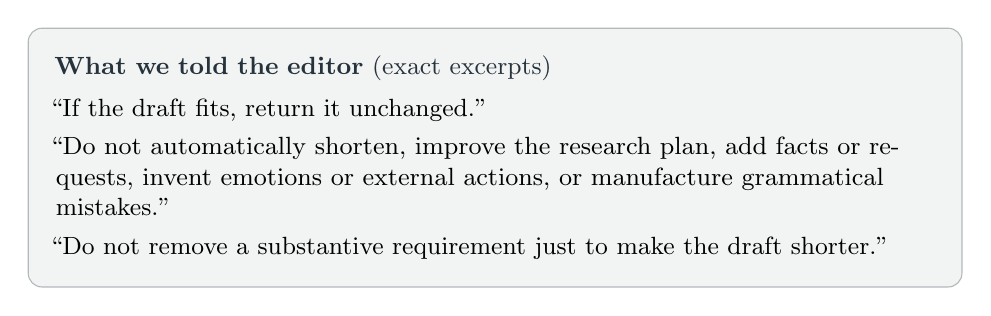
\begin{tikzpicture}[font=\small]
\node[draw=model!35,fill=model!6,rounded corners=5pt,inner sep=10pt,text width=.92\linewidth,align=left] (prompt) {
\textcolor{model}{\textbf{What we told the editor \normalfont(exact excerpts)}}\\[4pt]
``If the draft fits, return it unchanged.''\\[3pt]
``Do not automatically shorten, improve the research plan, add facts or requests, invent emotions or external actions, or manufacture grammatical mistakes.''\\[3pt]
``Do not remove a substantive requirement just to make the draft shorter.''};
\end{tikzpicture}

\caption{Excerpts from the Task 2 editor prompt, shown exactly as submitted.}\label{fig:prompt}
\end{figure}

\clearpage
\section{Results}
Our replies were longer than the human replies in both tasks (Figure~\ref{fig:results}). The organizers' November 4 release contains our annotated conversations, human ratings for some replies, and summary statistics for human conversations~\cite{results}. It does not include the human test replies themselves. Human training conversations were available separately.

\begin{figure}[H]\centering
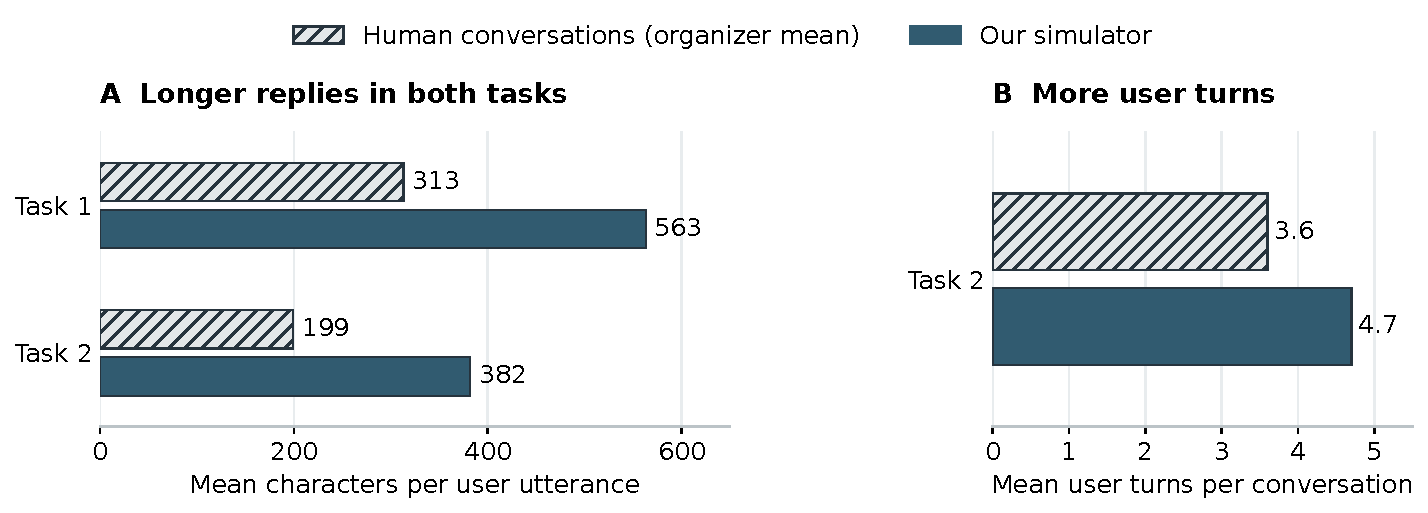
\includegraphics[width=\linewidth]{figures/results-comparison.pdf}
\caption{Average reply lengths and conversation lengths for our runs and the human comparison: 62 conversations in Task 1 and 57 in Task 2 per group. The release does not report how much these values vary across conversations. These bars show length; human-likeness ratings are in Table~\ref{tab:scores}.}\label{fig:results}
\end{figure}

Task 1 replies were about 80\% longer than the human mean; Task 2 replies were 92\% longer. Task 2 also averaged 4.7 researcher turns versus 3.6 for humans. More turns can be useful, so this difference alone does not show that the simulator should have stopped earlier.

\begin{table}[H]\centering\small
\begin{tabularx}{\linewidth}{@{}Yrr@{}}\toprule
Measure & Task 1 & Task 2\\\midrule
Dialogue-act JSD (lower is closer) & 0.106 & 0.158\\
Human-likeness mean (0--4) & 2.38 & 2.31\\
Rated user turns / conversations & 16 / 16 & 67 / 14\\\bottomrule
\end{tabularx}
\caption{Preliminary scores for our submitted runs. The organizers supplied JSD; we averaged the human ratings they provided. The human-likeness scale runs from definitely a bot (0) to definitely human (4).}\label{tab:scores}
\end{table}

Dialogue acts describe the type of conversational move. JSD (Jensen--Shannon divergence) measures how often our simulator uses these moves compared with humans: 0 means matching distributions and 1 means no overlap. Three LLMs assigned the labels by majority vote. The human ratings cover only the replies counted in Table~\ref{tab:scores}; some come from the same conversation. We received no human baseline rating or other teams' scores, so we cannot say how we rank.

We submitted 62 Task 1 predictions and processed 57 Task 2 conversations. Eight Task 2 conversations ended because of backend failures or timeouts. These were not the simulator's choices to stop. The organizers did not provide scores with those conversations removed.





\clearpage
\subsection{Two conversations with different ratings}
Figure~\ref{fig:comparison} shows one highly rated and one poorly rated Task 2 exchange about named-entity recognition (NER) datasets. The editor left all four shown replies unchanged.

\begin{figure}[H]\centering
\newcommand{\compareLeftFollow}{\notenum{1}\leadmark{Please provide the licensing, splits, and annotation provenance} for WikiANN and WikiNeural, especially whether their annotations are human-verified.}
\newcommand{\compareRightFollow}{\notenum{1}\leadmark{Thanks—this is a helpful shortlist, and I appreciate the caveats. I’m still hesitant to treat the license summaries as verified, since the answer points to project pages but doesn’t identify the exact release files or license documents.} Could you do one focused check for \notenum{2}\syntaxmark{**}MasakhaNER 2.0, HIPE-2020, and LitBank\syntaxmark{**}: give the precise release/repository location and state separately what terms apply to the annotations and to the underlying text? If a release has no clear license file or its terms are ambiguous, please say that explicitly rather than infer a license.}
\newcommand{\compareLeftClose}{\notenum{3}\goodmark{Thanks. That answers the question:} the index has no humanities-specific annotated NER corpus, so I’ll treat the multilingual general-domain datasets \goodmark{only as methodological benchmarks, not substitutes for humanities data.}}
\newcommand{\compareRightClose}{That distinction is exactly what I needed. I’ll treat the \notenum{3}\goodmark{release-level license statements as provisional} where the files don’t make their scope clear, and keep the annotation rights separate from the source-text rights. For now, LitBank looks like the clearest candidate for literary work, while HIPE and MasakhaNER are useful research resources but need \goodmark{version- and source-specific review before redistribution}. Thanks for correcting the earlier overstatement and making the remaining uncertainty explicit.}
\begin{minipage}{\linewidth}
\linespread{1.0}\selectfont
\small
\setlength{\tabcolsep}{7pt}
\renewcommand{\arraystretch}{1.0}
\begin{tabularx}{\linewidth}{@{}Y|Y@{}}
\textcolor{researcher}{\textbf{Better-rated conversation}} & \textcolor{error}{\textbf{Poorly rated conversation}}\\[6pt]
\searchicon\enspace\textbf{Assistant / summary} & \searchicon\enspace\textbf{Assistant / summary}\\[2pt]
Offers WikiANN and WikiNeural as multilingual options. Says the index has no ready-made annotated corpus specifically for humanities or historical text. & Recommends a shortlist including MasakhaNER, HIPE and LitBank. Gives project links and discusses annotation quality and licensing, while noting that exact release terms need checking.\\[5pt]\hline\noalign{\vskip4pt}
\simicon\enspace\textbf{Follow-up: 4/4; 148 characters} & \simicon\enspace\textbf{Follow-up: 0/4; 568 characters}\\[3pt]
\compareLeftFollow & \compareRightFollow\\[5pt]\hline\noalign{\vskip4pt}
{\footnotesize\color{gray}Three intervening exchanges omitted.} & {\footnotesize\color{gray}Next assistant reply; no exchanges omitted.}\\[3pt]
\searchicon\enspace\textbf{Assistant / summary} & \searchicon\enspace\textbf{Assistant / summary}\\[2pt]
Says none of the results in its index is a humanities-specific annotated NER dataset, and declines to offer raw historical text as an annotated substitute. & Acknowledges that earlier license summaries were not fully verified. Separates the rights in annotations from those in the source text and gives a qualified, release-by-release account.\\[5pt]\hline\noalign{\vskip4pt}
\simicon\enspace\textbf{Closing: 4/4; 220 characters} & \simicon\enspace\textbf{Closing: 1/4; 509 characters}\\[3pt]
\compareLeftClose & \compareRightClose\\[5pt]
\end{tabularx}
\par\vspace{7pt}
{\footnotesize
\textbf{1\quad How the request starts:} direct request versus two introductory sentences.\\[2pt]
\textbf{2\quad Visible markup:} the organizer-provided human rating cites ** and dash punctuation as bot-like cues.\\[2pt]
\textbf{3\quad What the closing emphasizes:} intended use versus repeated licensing qualifications.
}
\end{minipage}

\caption{Two selected examples. Gray highlights link to notes 1--3. We quote the simulator exactly, summarize assistant replies, and mark skipped exchanges. Ratings and note 2 come from the organizers' human evaluation; other notes are ours. These examples cannot show how common the behavior is or what caused the ratings. We did not check factual accuracy.}\label{fig:comparison}
\end{figure}

\clearpage
\section{Discussion}\label{sec:gaps}
We did a poor job of checking whether our simulator sounded like a person. We checked too few examples and reused training conversations. Looking back at the prompt and the official replies, we see two problems with how we used the editor.

\textbf{The editor usually copied the draft.} We told it to keep the details and avoid shortening replies automatically (Figure~\ref{fig:prompt}). That was a bad prompt for dealing with overly long replies. We gave it no length target based on human replies. Of 258 generated Task 2 draft/edit pairs, 245 (95\%) were unchanged, two became shorter, and eleven became longer. The editor therefore did little to change the length of our replies.

\textbf{We used our own replies as style examples.} In Task 2, the editor's examples were the simulator's last two messages. For the poorly rated closing in Figure~\ref{fig:comparison}, its input included this earlier reply:
\begin{quote}\small
\textcolor{researcher}{\textbf{Earlier reply, supplied as a voice reference:}} ``Thanks---this is a helpful shortlist, and I appreciate the caveats.''\par
\textcolor{model}{\textbf{Next closing draft, returned unchanged:}} ``That distinction is exactly what I needed.''
\end{quote}
Both replies start by thanking or agreeing with the assistant. We asked the editor to follow the simulator's earlier wording, so we may have encouraged it to keep a style that already sounded unnatural. We did not test whether human examples would work better. We also have no human ratings of the original drafts, so we cannot say whether the edits improved them.

\textbf{What we would do better.} We would give the editor examples of human wording from the training data, then compare drafts and edits on separate conversations. We would ask human raters whether each reply sounds natural and check that the edit keeps the request and uncertainty intact. Shortening a reply is useful only if it still says what the researcher meant.

\begin{thebibliography}{9}\small
\bibitem{track} TREC User Simulation Track organizers. \emph{Guidelines for Participants}. \url{https://trec.usersim.ai/guidelines}. Accessed November 7, 2026.
\bibitem{luna} OpenAI. \emph{GPT-6 Luna: model documentation}. \url{https://developers.openai.com/api/docs/models/gpt-6-luna}. Accessed November 7, 2026.
\bibitem{results} TREC User Simulation Track organizers. \emph{Preliminary evaluation results: README and run annotations}. Participant release, November 4, 2026. Downloaded November 7, 2026.
\bibitem{code} NP Labs. \emph{TREC UserSim 2026: simulator source and aggregate evidence}. Private repository. \url{https://github.com/npatta01/trec-usersim-2026}.
\end{thebibliography}
\end{document}
